%\documentclass[fleqn, letterpaper]{amsart}
\documentclass[letterpaper]{tufte-handout}
%\usepackage{times}
\usepackage{amsmath}
\usepackage{amssymb}
\usepackage{graphicx}
\usepackage{booktabs}
\usepackage{multirow}
\usepackage{listings}
\usepackage{epstopdf}
\usepackage{bm}
%\usepackage[left=1in]{geometry}

\newcommand{\R}{\mathcal{R}}
\newcommand{\E}{\text{E}}
\newcommand{\p}{p_{XY}}
\newcommand{\T}{^\text{T}}
\newcommand{\y}{\mathbf{y}}
\newcommand{\z}{\mathbf{z}}
\newcommand{\I}{\mathbf{I}}
\newcommand{\HH}{\mathbf{H}}
\newcommand{\A}{\mathbf{A}}
\newcommand{\GG}{\mathbf{G}}
\newcommand{\vech}{\mathbf{h}}
\newcommand{\uu}{\mathbf{u}}
\newcommand{\cyy}{\mathbf{C}_{yy}}
\newcommand{\cyz}{\mathbf{C}_{yz}}
\newcommand{\czz}{\mathbf{C}_{zz}}
\newcommand{\cuu}{\mathbf{C}_{uu}}
\newcommand{\cvv}{\mathbf{C}_{vv}}
\newcommand{\cpp}{\mathbf{C}_{\psi\psi}}
\renewcommand{\arraystretch}{1.5}
\renewcommand{\vec}[1]{\mathrm{#1}}

\title{Course Project --- ENCE689E Spring 2014}
\author{David Prentiss}

\begin{document}
\maketitle

The Famine Early Warning System Network (FEWSNET) project is a federally funded effort to monitor regional and global economies, food, and climate in order to provide advanced warning of humanitarian, food related disasters.
Among the many FEWSNET tools is a model of pastoral herds. This model\cite{fewsnet} is an aid to the analysis of food security in regions where pastoral livelihoods are prevalent. While it sees wide adoption among food security analysts, its statistical properties are not well investigated. Furthermore it may be possible to enhance this model with adaptive filtering techniques.

\section{Herd Dynamics Model}
The herd dynamics model predicts the size and demographic features of a hypothetical herd from season to season based on the previous season's rainfall amount and quality.
These demographic features are sub--groups related to sex and reproductive capacity where individuals are categorized as either adult female, newborn, young female, or young male.
As such, the state of the herd at each season $t$, where $t$ is an index of sequential seasons is captured by the state vector $\vech_t$.
The elements of $\vech_t$ are the head--counts of individuals in each sub--group at the beginning of season $t$.
That is
\begin{equation}
\vech_t = \begin{pmatrix} h_{AF} \\ h_{NM} \\ h_{YF} \\ h_{YM} \end{pmatrix}
\end{equation}
where $h_{AF}$, $h_{NM}$, $h_{YF}$, $h_{YM}$ are the number of adult female, newborn, young female, or young male individuals respectively.
Individuals are added to each sub--group as they are born or graduate from one sub--group to another; they are removed as they die, are sold, or graduate.

The rates at which individuals are added or removed is assumed to be a function of rainfall as represented by satellite based rainfall estimate $r_e^t$ during season $t$. The relationship between each rate and rainfall input is interpolated from empirical data. Figure \ref{rferels} illustrates the relevant relationships. The element-wise, discrete propagation step is
\begin{align}
  h_{AF}^{t+1} &= h_{AF}^t + h_{YF}^t - f_{SF}h_{AF}^t - f_{MM}h_{AF}^t \\
  h_{NB}^{t+1} &= f_{C}h_{AF}^t \\
  h_{YF}^{t+1} &= 0.5(h_{NB}^t - f_{MI}h_{NB}^t) - f_{MM}h_{YF}^t \\
  h_{YM}^{t+1} &= h_{YM}^t + h_{NB}^t - h_{YF}^{t+1} - f_{SM}h_{YM}^t - f_{MM}h_{YM}^t
\end{align}
where $f_{C}$, $f_{SM}$, $f_{SF}$, $f_{MM}$, and $f_{MI}$ are the rates of conception, male sales, female sales, mature mortality, and immature mortality for rainfall $r^t_e$ respectively. Step super--scipts and arguments have been omitted for clarity.
See figure \ref{rferels}.

\begin{figure}
  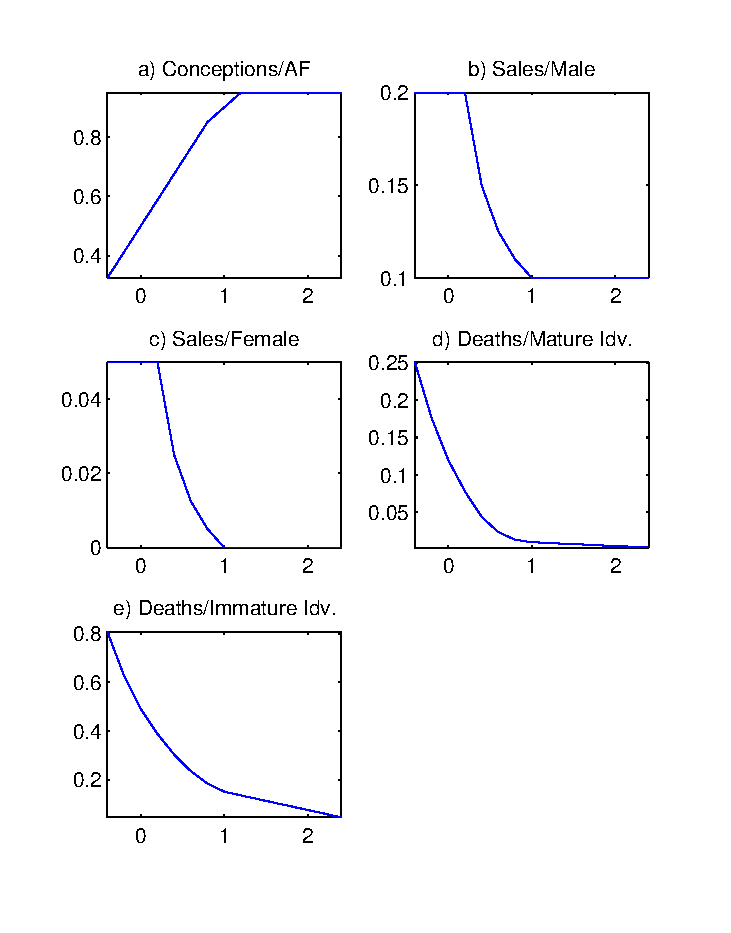
\includegraphics[width=\textwidth]{refrel}
  \caption{The relationship between various herd dynamic rates and rainfall. In each graph, the $x$ axis is seasonal rainfall normalized by the regional average and the $y$ axis is the respective change in herd demographic sub--group normalized by current population.}
  \label{rferels}
\end{figure}

\section{The Forward Model}

To begin analyzing the herd dynamics model, a 100-member ensemble was initialized with uncorrelated, uniformly distributed initial values. This ensemble was propagated for 100 steps for a variety of simulated rainfall time--series. These series were generated with a Gaussian random walk with mean 0 and variance 0.05. Figure \ref{rfe} illustrates one such series, figure \ref{ensemble} graph total herd size for the ensemble for 100 seasons, and listing \ref{code} is the code used to propagate the forward model.

\begin{figure}
  \includegraphics[width=\textwidth]{rfe}
  \caption{Rainfall realization generated by random walk}
  \label{rfe}
\end{figure}
\begin{figure}
  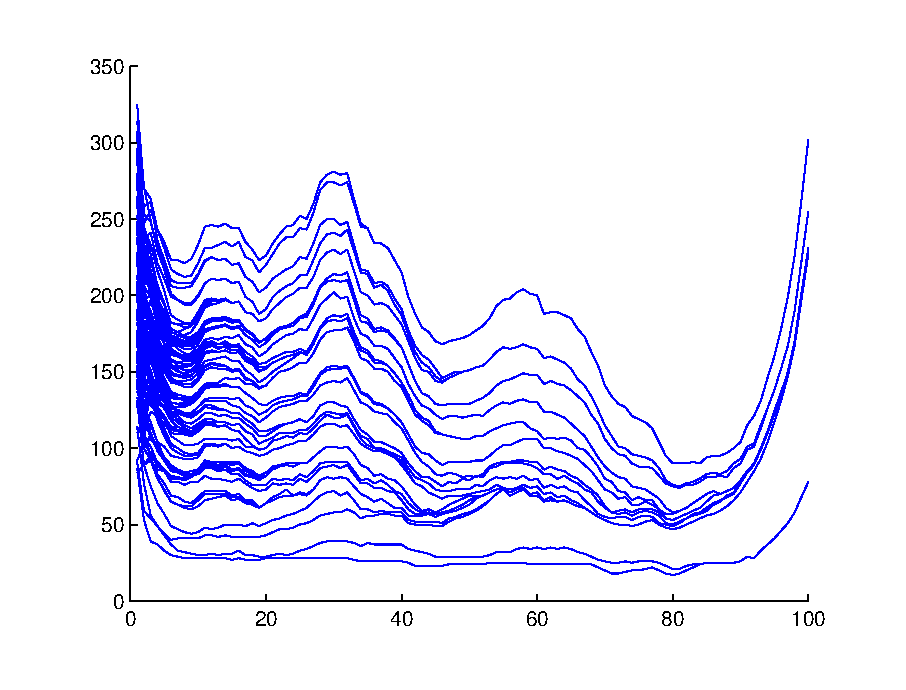
\includegraphics[width=\textwidth]{herdsize}
  \caption{Herd sizes of a 100-member ensemble propagated over 100 seasons.}
  \label{ensemble}
\end{figure}

\newpage
{\scriptsize
  \lstinputlisting[language=Matlab, caption={Herd ensemble forward model},
  basicstyle=\ttfamily, label=lst1]{herd.m}
  \label{code}
}

\bibliography{project}
\bibliographystyle{plainnat}

\end{document}
